\documentclass[12pt]{article}
\usepackage{graphicx} % Required for 
\usepackage[portuguese]{babel}
\usepackage{subfigure}
\usepackage{xcolor}
\usepackage{pdfpages}
\usepackage{booktabs} 
\usepackage{hyperref}
\usepackage{rotating}
\usepackage{amssymb}
\usepackage[top=3cm, right=3cm, left=3cm, right=3cm]{geometry}
\usepackage{enumitem}
\definecolor{codegreen}{rgb}{0,0.6,0}
\definecolor{codegray}{rgb}{0.5,0.5,0.5}
\definecolor{codepurple}{rgb}{0.58,0,0.82}
\definecolor{backcolour}{rgb}{0.95,0.95,0.92}


\author{Rodrigo José Zonzin Esteves}
\date{Junho de 2025}
\title{Prática 6 - Compêndio de Resultados - PSO}

\begin{document}
	\maketitle
	
	\section{Função objetivo}
	A função a ser otimizada é a função de Ackley 10-dimensional, $f: \mathbb{R}^{10} \mapsto \mathbb{R}$. 
	
	
	\section{Otimização dos parâmetros $k$, $m$ e $w$ }
	
	A Figura \ref{fig_variacaoiteracoes} apresenta 5 ensaios para diferentes valores de iteração máxima. \\
	$k \in~\{10, 20, 50, 100, 200, 500, 1000, 2000\}$.
	
	Como se observa, após a iteração 200 há poucas curvas que apresentaram alguma melhora no valor de \textit{fitness}. Para a Função Objetivo em tela esse resultado é esperado. 	
	\begin{figure}[h!]
		\centering
		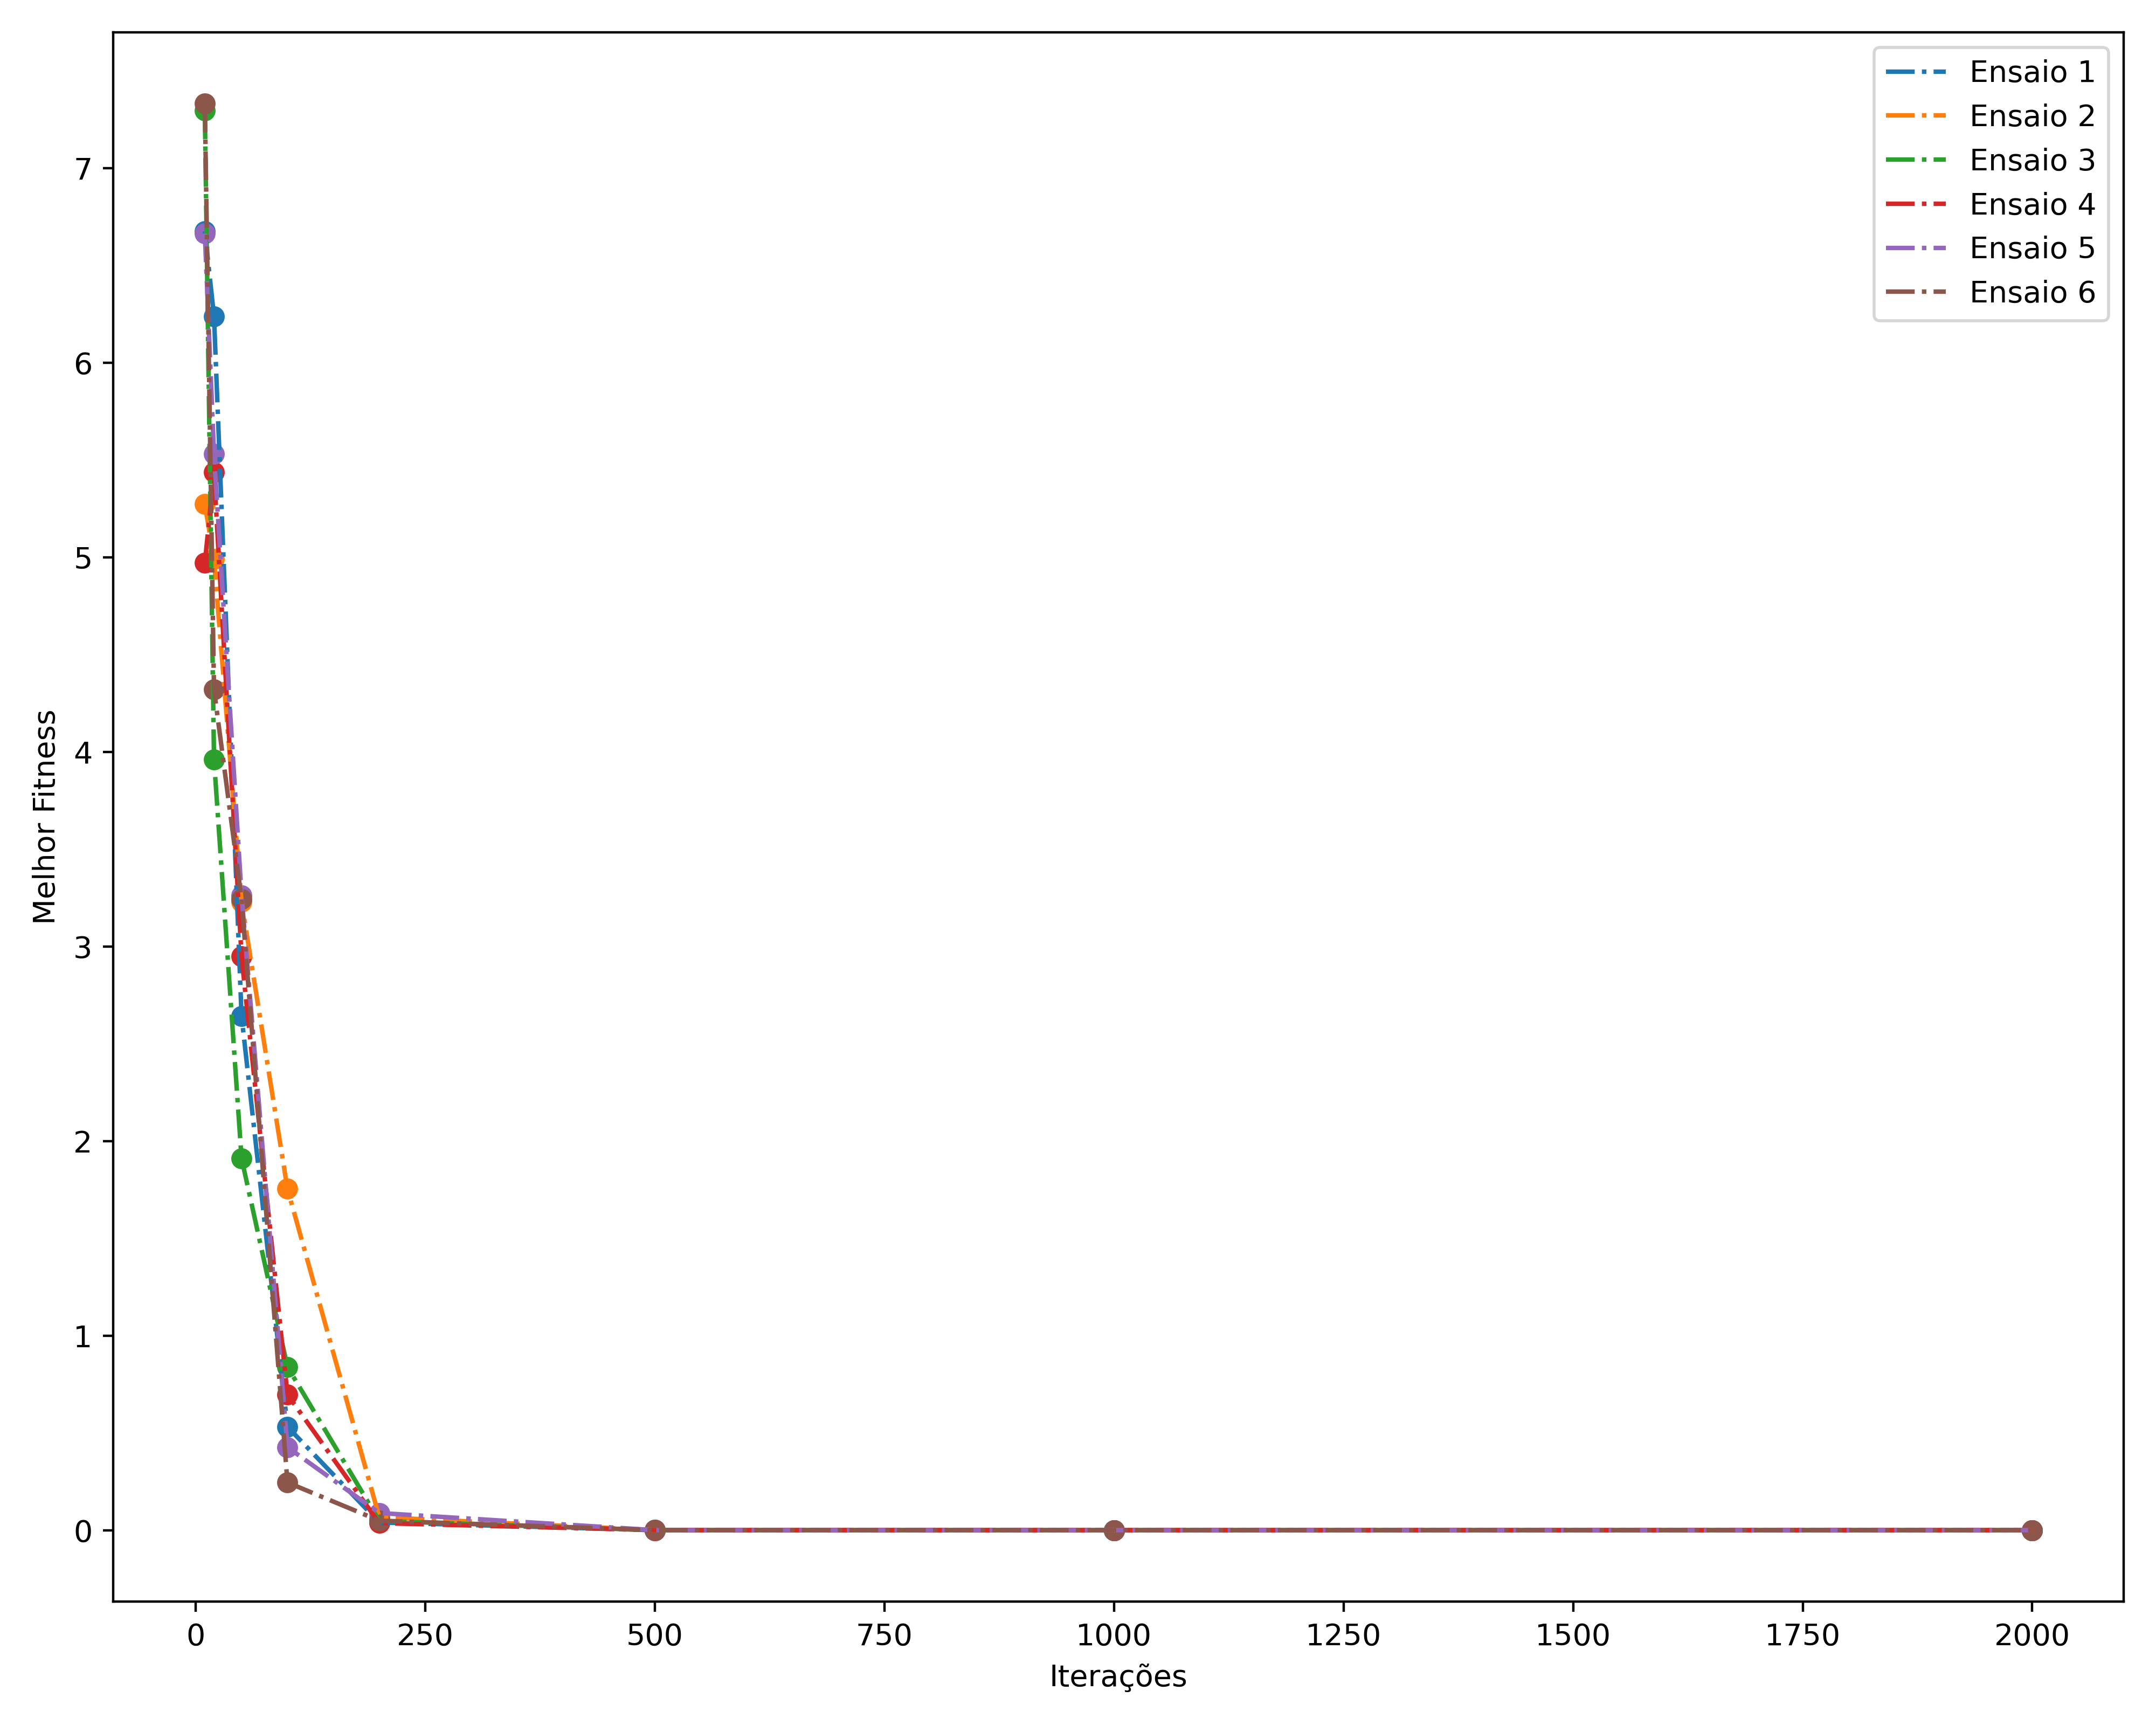
\includegraphics[width=0.68\linewidth]{../variacao_iteracoes}
		\caption{Comparação de número máximo de iterações e melhor \textit{fitness} obtido}
		\label{fig_variacaoiteracoes}
	\end{figure}
	 Apesar de a dimensionalidade da função ser mais alta em relação às abordagens das práticas anteriores, dez dimensões ainda não são suficientes para exigir mais avaliações do processo de otimização. Ele é simples. 
	
	Por essa razão, optou-se por estabelecer $k=500$ como um critério de parada geral. Essa escolha se justifica pois alcança o mínimo necessário para a otimização global e ainda apresenta uma margem considerável para processos eventualmente mais complexos. 
	
	Para a análise do número de partículas, optou-se por reduzir o total de iterações para $k=150$. Isso ocorre para que o estresse deste parâmetro no processo de otimização torne claro o impacto dos demais parâmetros na execução do algoritmo. A Figura \ref{fig_variandom} apresenta os resultados obtidos. 
	 
	\begin{figure}[h]
		\centering
		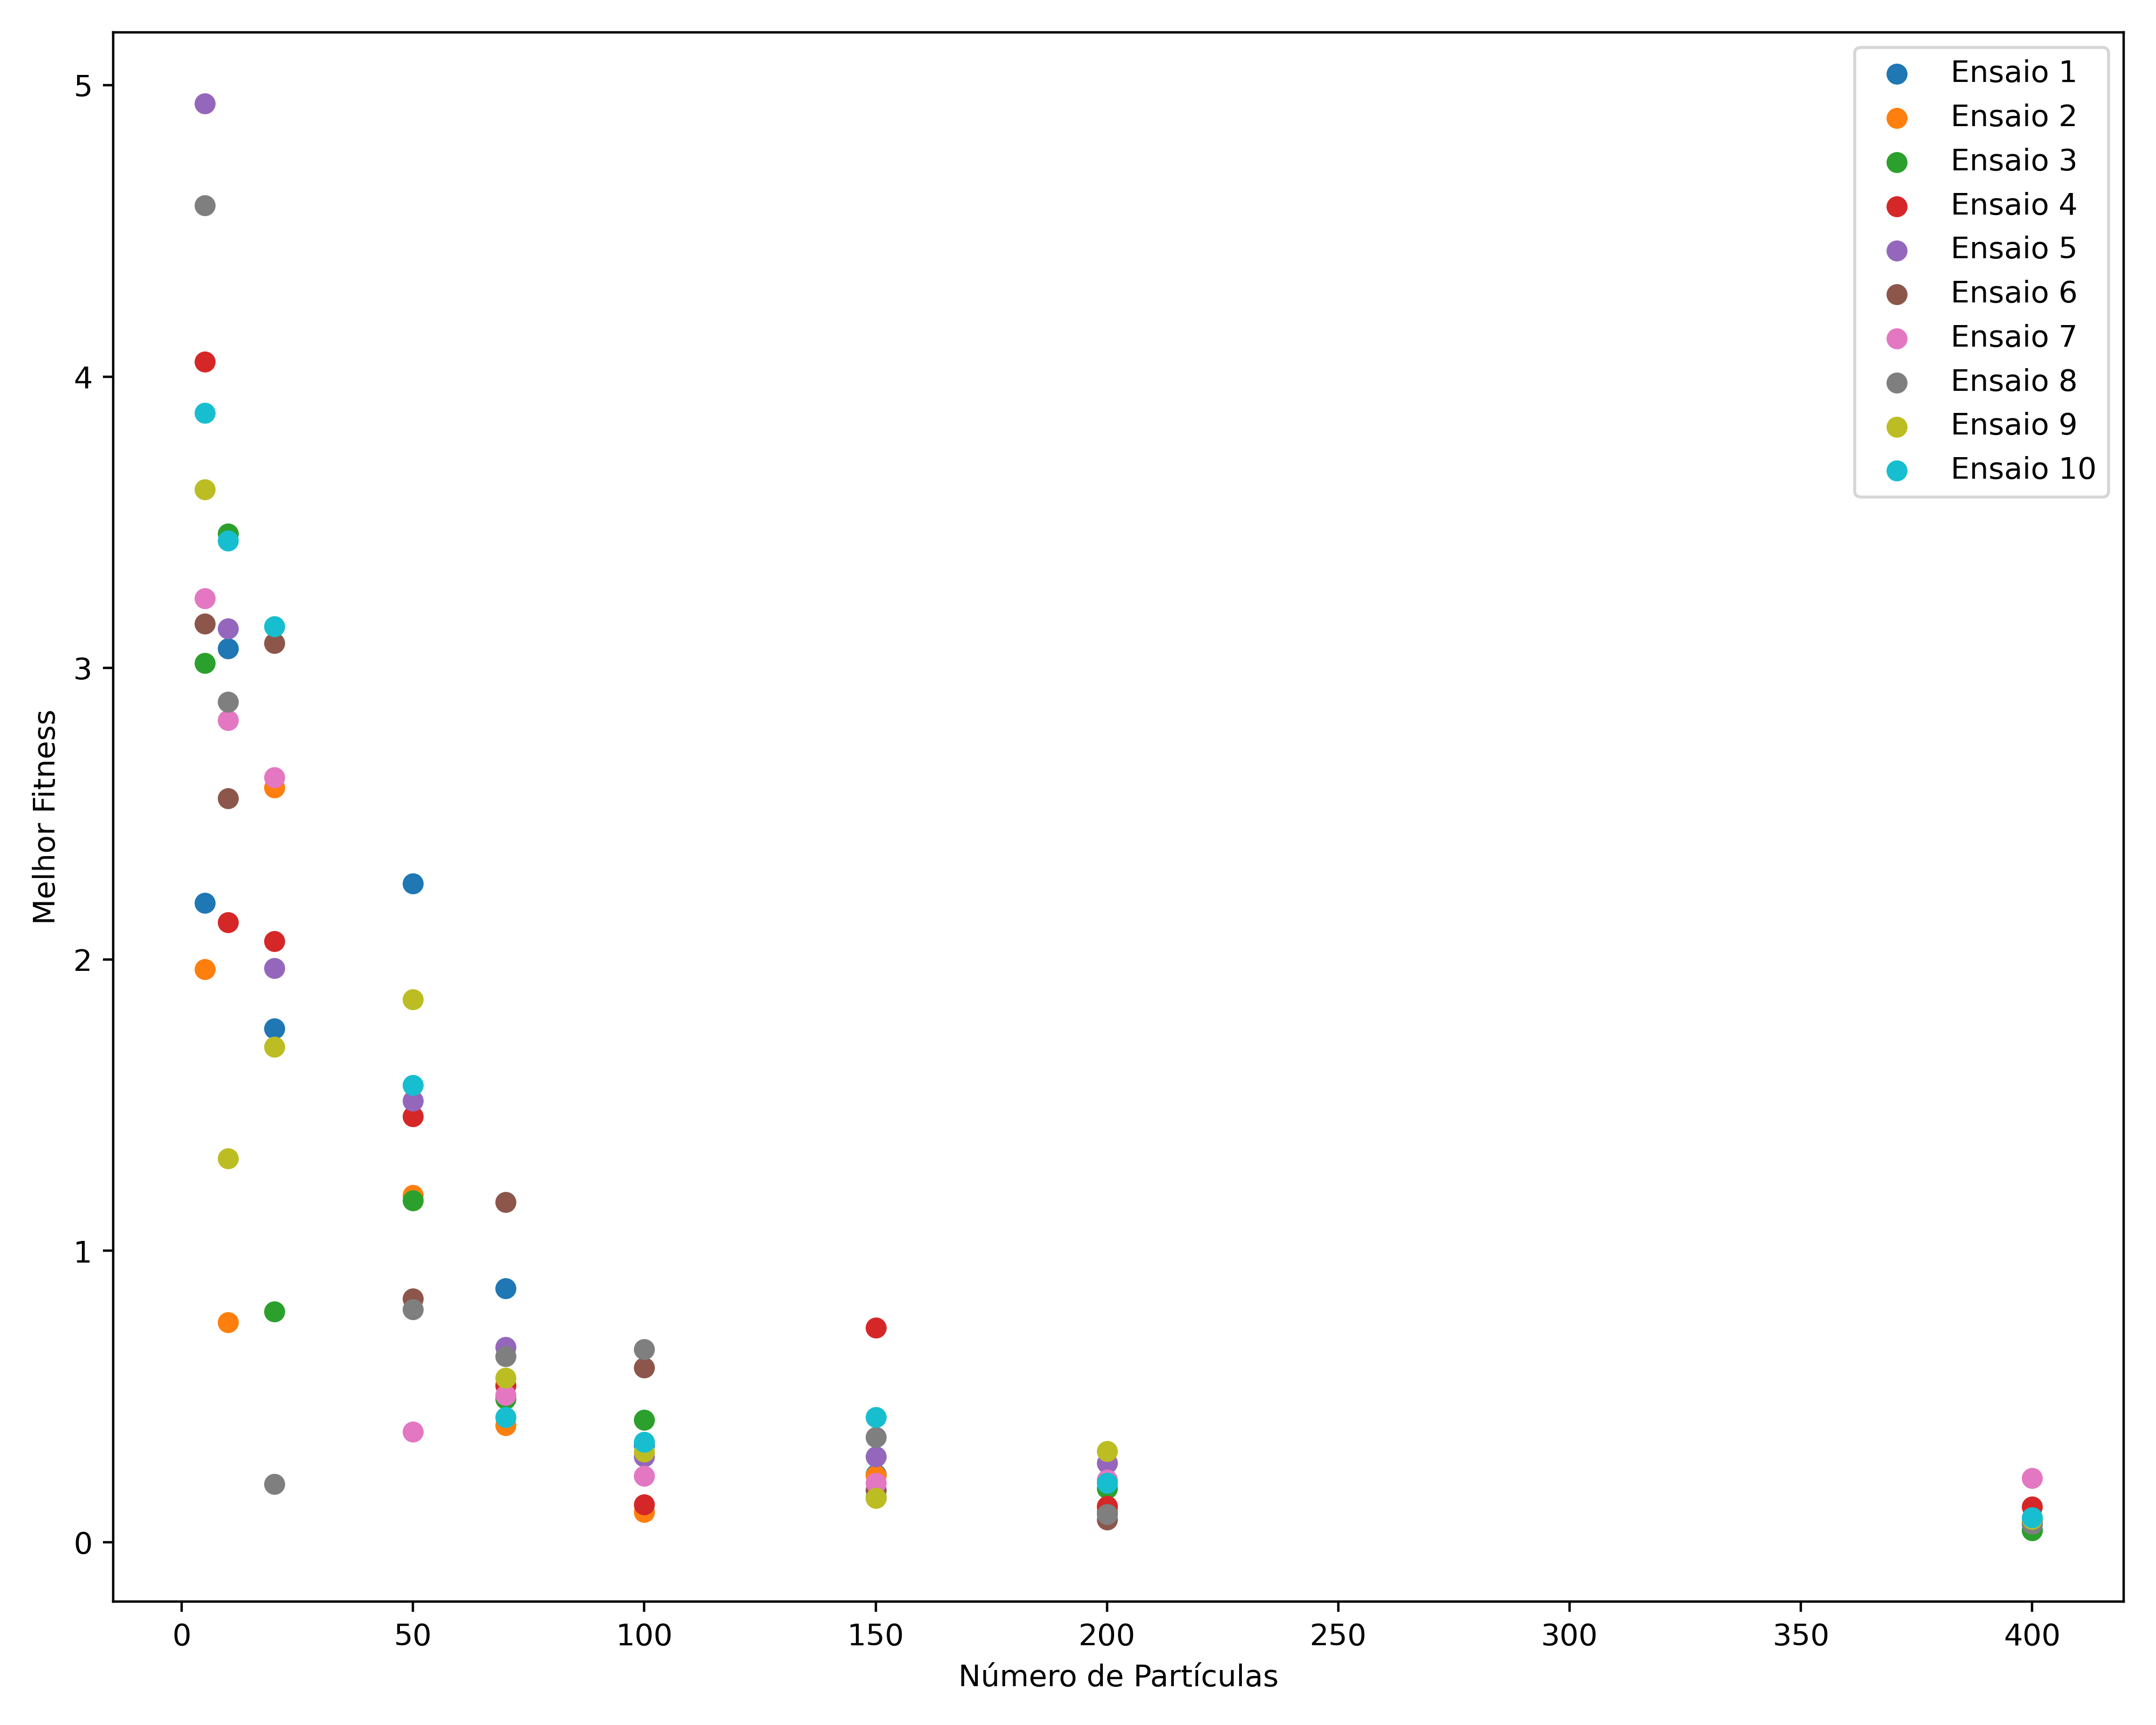
\includegraphics[width=0.7\linewidth]{../variando_m}
		\caption{Impacto do tamanho do enxame na obtenção do ótimo}
		\label{fig_variandom}
	\end{figure}
	A partir de 100 partículas, o algoritmo se estabiliza e os dados são significantes para sugerir que não uma melhora considerável para os parâmetros testados. Esse resultado é útil para se estabelecer um teto para $m$. Portanto, em primeiro momento, sugere-se $m \leq 200$. Essa análise, no entanto, é insuficiente para fixar um valor razoável de $m$: valores menores são suficientes para o propósito do trabalho desde que haja uma maior quantidade de iterações. 
	
	Para uma comparação mais aprofundada, a Figura \ref{fig_heatmapfitness} apresenta o melhor \textit{fitness} em função do número de iterações e do tamanho da população. 
	\begin{figure}[h!]
		\centering
		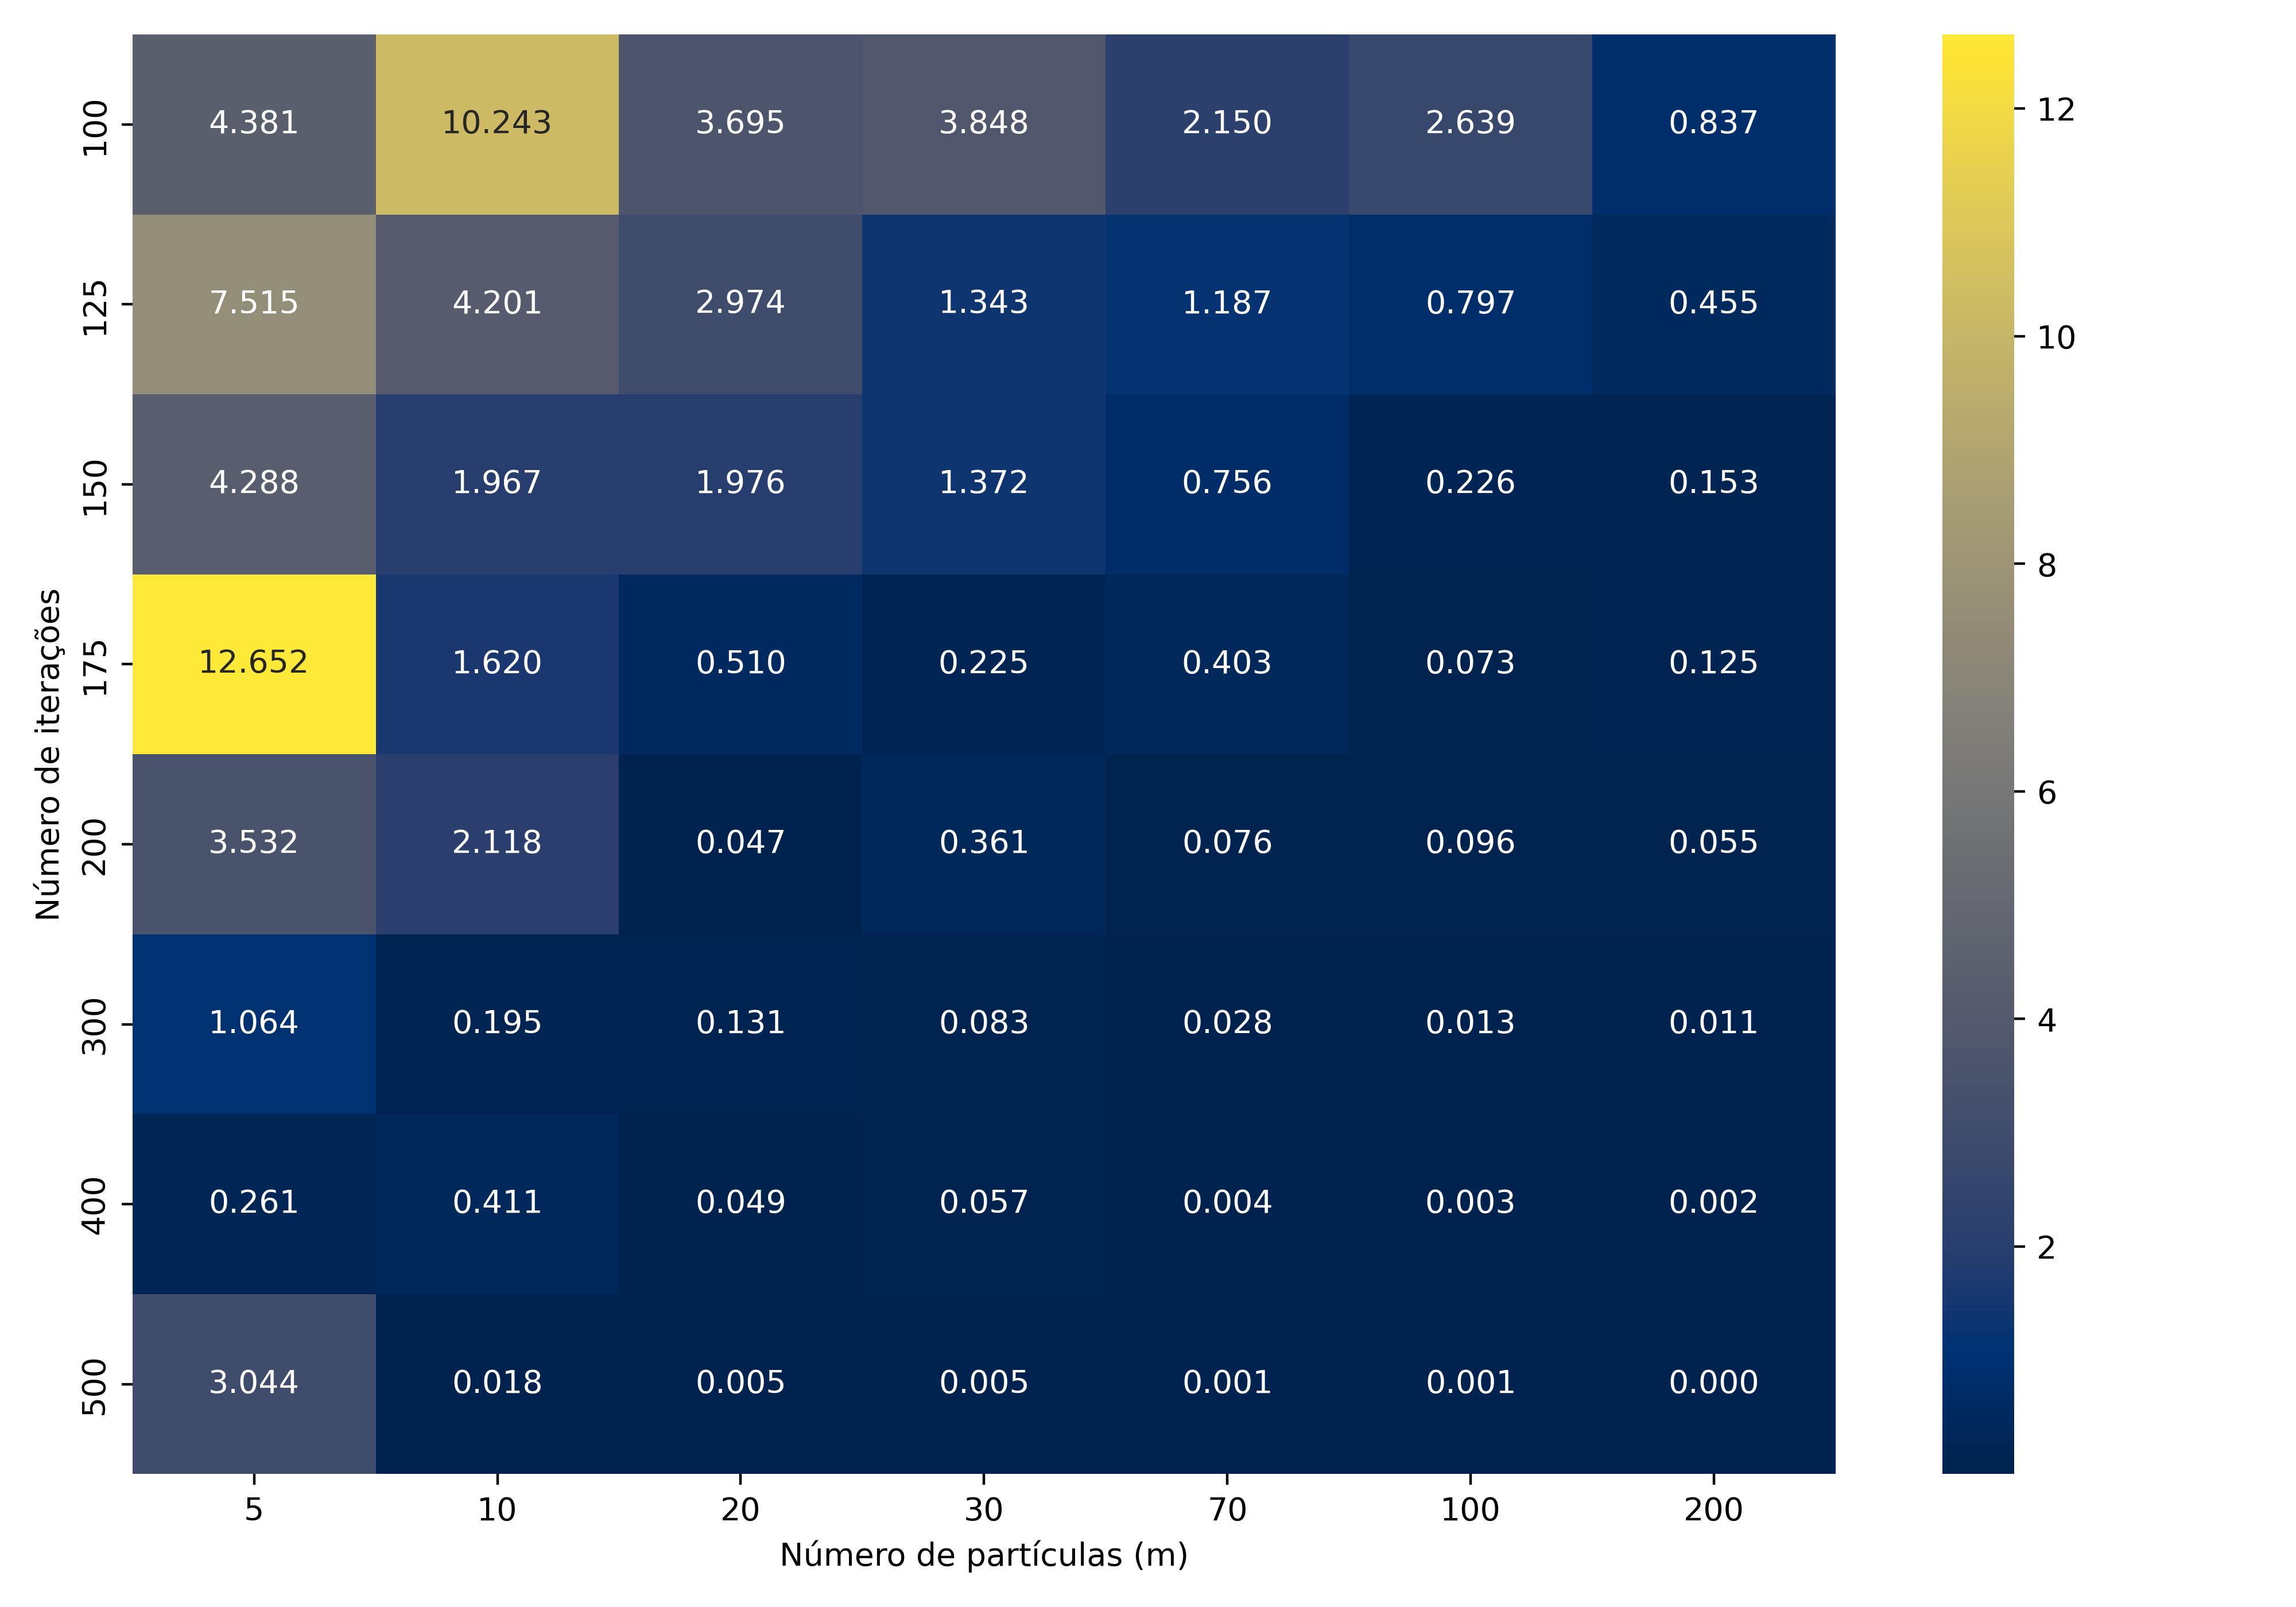
\includegraphics[width=0.7\linewidth]{../heatmap_fitness_novo}
		\caption{Heatmap do melhor \textit{fitness}, $k$ e $m$}
		\label{fig_heatmapfitness}
	\end{figure}
	
	Como se observa, para $k \geq 200$, 20 partículas já são suficientes para se obter uma boa aproximação para os zeros da função objetivo. Para $k=300$, o erro da aproximação é menor que $0.1$ em todos os casos examinados. Dessa maneira, mantém-se $k=500$ e se sugere $  20 \leq m \leq 70 $ como parâmetros gerais. 
	
\end{document}